\documentclass[12pt]{beamer}
\usepackage{../Estilos/BeamerFC}
\usepackage{../Estilos/ColoresLatex}
\usepackage{courier}
\usepackage{listingsutf8}
\usepackage{listings}
\usepackage{xcolor}
\usepackage{textcomp}
\usepackage{color}
\definecolor{deepblue}{rgb}{0,0,0.5}
\definecolor{brown}{rgb}{0.59, 0.29, 0.0}
\definecolor{OliveGreen}{rgb}{0,0.25,0}
% \usepackage{minted}

\DeclareCaptionFont{white}{\color{white}}
\DeclareCaptionFormat{listing}{\colorbox{gray}{\parbox{0.98\textwidth}{#1#2#3}}}
\captionsetup[lstlisting]{format=listing,labelfont=white,textfont=white}
\renewcommand{\lstlistingname}{Código}


\definecolor{Code}{rgb}{0,0,0}
\definecolor{Keywords}{rgb}{255,0,0}
\definecolor{Strings}{rgb}{255,0,255}
\definecolor{Comments}{rgb}{0,0,255}
\definecolor{Numbers}{rgb}{255,128,0}

\makeatletter

\newif\iffirstchar\firstchartrue
\newif\ifstartedbyadigit
\newif\ifprecededbyequalsign

\newcommand\processletter
{%
  \ifnum\lst@mode=\lst@Pmode%
    \iffirstchar%
        \global\startedbyadigitfalse%
      \fi
      \global\firstcharfalse%
    \fi
}

\newcommand\processdigit
{%
  \ifnum\lst@mode=\lst@Pmode%
      \iffirstchar%
        \global\startedbyadigittrue%
      \fi
      \global\firstcharfalse%
  \fi
}

\lst@AddToHook{OutputOther}%
{%
  \lst@IfLastOtherOneOf{=}
    {\global\precededbyequalsigntrue}
    {}%
}

\lst@AddToHook{Output}%
{%
  \ifprecededbyequalsign%
      \ifstartedbyadigit%
        \def\lst@thestyle{\color{orange}}%
      \fi
    \fi
  \global\firstchartrue%
  \global\startedbyadigitfalse%
  \global\precededbyequalsignfalse%
}

\lstset{ 
language=Python,                % choose the language of the code
basicstyle=\footnotesize\ttfamily,       % the size of the fonts that are used for the code
numbers=left,                   % where to put the line-numbers
numberstyle=\scriptsize,      % the size of the fonts that are used for the line-numbers
stepnumber=1,                   % the step between two line-numbers. If it is 1 each line will be numbered
numbersep=5pt,                  % how far the line-numbers are from the code
backgroundcolor=\color{white},  % choose the background color. You must add \usepackage{color}
showspaces=false,               % show spaces adding particular underscores
showstringspaces=false,         % underline spaces within strings
showtabs=false,                 % show tabs within strings adding particular underscores
frame=single,   		% adds a frame around the code
tabsize=2,  		% sets default tabsize to 2 spaces
captionpos=t,   		% sets the caption-position to bottom
breaklines=true,    	% sets automatic line breaking
breakatwhitespace=false,    % sets if automatic breaks should only happen at whitespace
escapeinside={| |},  % if you want to add a comment within your code
stringstyle =\color{OliveGreen},
otherkeywords={as, np.array, np.concatenate, np.linspace, linspace, interpolate.interp1d, kind, plt.plot, .copy, np.arange, np.cos, np.pi, lw, ls, label, splrep, splev, plt.legend, loc, plt.title, plt.ylim, plt.show, sign, math.ceil, math.log, np.sqrt, np.exp, np.zeros, plt.xlabel, plt.ylabel, plt.xlim, np.identity, random, np.dot, np.outer, np.diagonal },             % Add keywords here
keywordstyle = \color{blue},
commentstyle = \color{darkcerulean},
identifierstyle = \color{black},
literate=%
         {á}{{\'a}}1
         {é}{{\'e}}1
         {í}{{\'i}}1
         {ó}{{\'o}}1
         {ú}{{\'u}}1
%
%keywordstyle=\ttb\color{deepblue}
%fancyvrb = true,
}

\lstdefinestyle{FormattedNumber}{%
    literate={0}{{\textcolor{red}{0}}}{1}%
             {1}{{\textcolor{red}{1}}}{1}%
             {2}{{\textcolor{red}{2}}}{1}%
             {3}{{\textcolor{red}{3}}}{1}%
             {4}{{\textcolor{red}{4}}}{1}%
             {5}{{\textcolor{red}{5}}}{1}%
             {6}{{\textcolor{red}{6}}}{1}%
             {7}{{\textcolor{red}{7}}}{1}%
             {8}{{\textcolor{red}{8}}}{1}%
             {9}{{\textcolor{red}{9}}}{1}%
             {.0}{{\textcolor{red}{.0}}}{2}% Following is to ensure that only periods
             {.1}{{\textcolor{red}{.1}}}{2}% followed by a digit are changed.
             {.2}{{\textcolor{red}{.2}}}{2}%
             {.3}{{\textcolor{red}{.3}}}{2}%
             {.4}{{\textcolor{red}{.4}}}{2}%
             {.5}{{\textcolor{red}{.5}}}{2}%
             {.6}{{\textcolor{red}{.6}}}{2}%
             {.7}{{\textcolor{red}{.7}}}{2}%
             {.8}{{\textcolor{red}{.8}}}{2}%
             {.9}{{\textcolor{red}{.9}}}{2}%
             {\ }{{ }}{1}% handle the space
         ,%
          %mathescape=true
          escapeinside={__}
          }



\usepackage[siunitx]{circuitikz}
\usetikzlibrary{arrows,patterns,shapes}
\usetikzlibrary{decorations.markings}
\usetikzlibrary{arrows}
\usetheme{Copenhagen}
\usecolortheme{wolverine}
%\useoutertheme{default}
\setbeamercovered{invisible}
% or whatever (possibly just delete it)
\setbeamertemplate{section in toc}[sections numbered]
\setbeamertemplate{subsection in toc}[subsections numbered]
\setbeamertemplate{subsection in toc}{\leavevmode\leftskip=3.2em\rlap{\hskip-2em\inserttocsectionnumber.\inserttocsubsectionnumber}\inserttocsubsection\par}
% \setbeamercolor{section in toc}{fg=blue}
% \setbeamercolor{subsection in toc}{fg=blue}
% \setbeamercolor{frametitle}{fg=blue}
\setbeamertemplate{caption}[numbered]

\setbeamertemplate{footline}
\beamertemplatenavigationsymbolsempty
\setbeamertemplate{headline}{}


\makeatletter
% \setbeamercolor{section in foot}{bg=gray!30, fg=black!90!orange}
% \setbeamercolor{subsection in foot}{bg=blue!30}
% \setbeamercolor{date in foot}{bg=black}
\setbeamertemplate{footline}
{
  \leavevmode%
  \hbox{%
  \begin{beamercolorbox}[wd=.333333\paperwidth,ht=2.25ex,dp=1ex,center]{section in foot}%
    \usebeamerfont{section in foot} \insertsection
  \end{beamercolorbox}%
  \begin{beamercolorbox}[wd=.333333\paperwidth,ht=2.25ex,dp=1ex,center]{subsection in foot}%
    \usebeamerfont{subsection in foot}  \insertsubsection
  \end{beamercolorbox}%
  \begin{beamercolorbox}[wd=.333333\paperwidth,ht=2.25ex,dp=1ex,right]{date in head/foot}%
    \usebeamerfont{date in head/foot} \insertshortdate{} \hspace*{2em}
    \insertframenumber{} / \inserttotalframenumber \hspace*{2ex} 
  \end{beamercolorbox}}%
  \vskip0pt%
}
\makeatother

\makeatletter
\patchcmd{\beamer@sectionintoc}{\vskip1.5em}{\vskip0.8em}{}{}
\makeatother

% %\newlength{\depthofsumsign}
% \setlength{\depthofsumsign}{\depthof{$\sum$}}
% \newcommand{\nsum}[1][1.4]{% only for \displaystyle
%     \mathop{%
%         \raisebox
%             {-#1\depthofsumsign+1\depthofsumsign}
%             {\scalebox
%                 {#1}
%                 {$\displaystyle\sum$}%
%             }
%     }
% }
% \def\scaleint#1{\vcenter{\hbox{\scaleto[3ex]{\displaystyle\int}{#1}}}}
% \def\scaleoint#1{\vcenter{\hbox{\scaleto[3ex]{\displaystyle\oint}{#1}}}}
% \def\bs{\mkern-12mu}

\usefonttheme{serif}

\title{\large{EDO con CDF - Solución}}
\subtitle{Tema 3 - Ecuaciones Diferenciales Ordinarias}
\author{M. en C. Gustavo Contreras Mayén}
\date{}

\begin{document}
\maketitle

\section{Resolviendo las ED CDF}
\frame{\tableofcontents[currentsection, hideothersubsections]}
\subsection{Ejercicio 1}

\begin{frame}
\frametitle{Enunciado del Ejercicio}
Para el siguiente problema de una ED lineal con CDF:
\pause
\begin{align*}
\sderivada{y} = - 4 \, y + 4 \, x \hspace{1cm} y (0) = 0 \hspace{0.5cm} \pderivada{y} (\pi/2) = 0
\end{align*}
\pause
\setbeamercolor{item projected}{bg=blue-green,fg=bole}
\setbeamertemplate{enumerate items}{%
\usebeamercolor[bg]{item projected}%
\raisebox{1.5pt}{\colorbox{bg}{\color{fg}\footnotesize\insertenumlabel}}%
}
\begin{enumerate}[<+->]
\item Escribe el sistema de ecuaciones algebraicas, considera el valor de $m = 10$
\item Resuelve el sistema anterior.
\end{enumerate}
\end{frame}
\begin{frame}
\frametitle{Resolviendo el primer inciso}
En este caso, tenemos que:
\pause
\begin{align*}
\alpha &= y (0) = 0 \\
\beta &= \pderivada{y} (\pi/2) = 0 \\
f (x, y, \pderivada{y}) &= - 4 \, y + 4 \, x
\end{align*}
\end{frame}
\begin{frame}
\frametitle{Sistema de ecuaciones algebraicas}
Tenemos entonces:
\pause
\begin{align*}
y_{0} =& \, 0 \\
y_{i-1} - 2 \, y_{i} + y_{i+1} - h^{2} (- 4 \, y_{i} + 4 \, x_{i}) =& \, 0 \\
2 \, y_{9} - 2 \, y_{10} - h^{2} (- 4 \, y_{10} + 4 \, x_{10}) =& \, 0 \\
i = 1, 2, \ldots, &m - 1
\end{align*}
\end{frame}
\begin{frame}
\frametitle{Representación matricial}
\begin{align*}
\begingroup % keep the change local
\setlength\arraycolsep{2pt}
\begin{bmatrix}
1 & 0 & & & & \\
1 & -2 + 4 h^{2} & 1 & & \\
 & \ddots & \ddots & \ddots & \\
 & & 1 & -2 + 4 h^{2} & 1 \\
 & & & 2 & -2 + 4 h^{2}
\end{bmatrix}
\endgroup
\begin{bmatrix}
y_{0} \\
y_{1} \\
\vdots \\
y_{m-1} \\
y_{m1} \
\end{bmatrix}
=
\begin{bmatrix}
0 \\
4 h^{2} x_{1} \\
\vdots \\
4 h^{2} x_{m-1} \\
4 h^{2} x_{m}
\end{bmatrix}
\end{align*}
\end{frame}
\begin{frame}
\frametitle{Del sistema anterior}
Del sistema anterior, encontramos que la \textbf{\textcolor{bondiblue}{matriz de coeficientes}} es \textbf{\textcolor{cadet}{tridiagonal}}.
\\
\bigskip
\pause
Por lo que las ecuaciones se pueden resolver de manera eficiente mediante las rutinas de descomposición y sustitución como se verá a continuación.
\end{frame}

\section{Métodos de descomposición LU}
\frame{\tableofcontents[currentsection, hideothersubsections]}
\subsection{Definición}

\begin{frame}
\frametitle{Métodos de descomposición \textbf{LU}}
Se puede demostrar que cualquier matriz cuadrada $\mathbf{A}$ se puede expresar como un producto de una matriz triangular inferior $\mathbf{L}$ y una matriz triangular superior $\mathbf{U}$:
\pause
\begin{align*}
\mathbf{A = L \: U}
\end{align*}
\end{frame}
\begin{frame}
\frametitle{Factorización \textbf{LU}}
El proceso de calcular $\mathbf{L}$ y $\mathbf{U}$ para un determinada matriz $\mathbf{A}$, se conoce como \textbf{\textcolor{blue}{descomposición LU}} \pause o \textbf{\textcolor{blue}{factorización LU}}.
\end{frame}
\begin{frame}
\frametitle{Descomposición $LU$}
La descomposición $\mathbf{LU}$ no es única \pause (las combinaciones de $\mathbf{L}$ y $\mathbf{U}$ para una determinada matriz A son infinitas), salvo ciertas restricciones de $\mathbf{L}$ o $\mathbf{U}$. 
\\
\bigskip
Estas limitaciones distinguen un tipo de descomposición de otro.
\end{frame}

\subsection{Métodos más utilizados}

\begin{frame}
\frametitle{Métodos $LU$ más utilizados}
Los tres métodos de descomposición $LU$ más utilizados son:
\pause
\begin{table}[H]
\centering
\begin{tabular}{l | l}
Nombre & Restricciones \\ \hline
Doolittle & $L_{ii} = 1, \hspace{0.3cm} i = 1, 2, \ldots, n$ \\
Crout & $U_{ii} = 1, \hspace{0.3cm} i = 1, 2, \ldots, n$ \\
Choleski & $L = U^{T}$ 
\end{tabular}
\end{table}
\end{frame}
\begin{frame}
\frametitle{Versatilidad de los métodos}
Después de descomponer a $\mathbf{A}$, se facilita resolver las ecuaciones $\mathbf{A} \: x = \mathbf{b}$. 
\\
\bigskip
\pause
En primer lugar, volvemos a escribir las ecuaciones como $\mathbf{L} \: \mathbf{U} \: x = \mathbf{b}$.
\end{frame}
\begin{frame}
\frametitle{Versatilidad de los métodos}
Al usar la notación $\mathbf{U} \: x = \mathbf{y}$, las ecuaciones quedan como:
\pause
\begin{align*}
\mathbf{L \: y = b}
\end{align*}
que se puede resolver para $y$ por sustitución hacia delante. 
\end{frame}
\begin{frame}
\frametitle{Versatilidad de los métodos}
Entonces:
\pause
\begin{align*}
\mathbf{U \: x = y}
\end{align*}
nos devolverá $x$ con el proceso de sustitución hacia atrás.
\end{frame}
\begin{frame}
\frametitle{Versatilidad de los métodos}
La ventaja de la descomposición $LU$ sobre el método de eliminación de Gauss es que una vez descompuesta, podemos resolver $\mathbf{A} \, x = \mathbf{b}$ para muchos vectores constantes $b$.
\end{frame}
\begin{frame}
\frametitle{Versatilidad de los métodos}
El costo de cada solución adicional es relativamente pequeño, ya que el avance y las operaciones de sustitución están consumiendo mucho menos tiempo que el proceso de descomposición.
\end{frame}

\section{Descomposición de Doolittle}
\frame{\tableofcontents[currentsection, hideothersubsections]}
\subsection{Descripción del método}

\begin{frame}
\frametitle{Descomposición de Doolittle}
El método de descomposición de Doolittle está estrechamente relacionado con el proceso de eliminación de Gauss.
\\
\bigskip
\pause
Veamos el método con un ejemplo:
\end{frame}
\begin{frame}[fragile]
\frametitle{Descomposición de Doolittle}
Considera una matriz $\mathbf{A}$ de $3 \times 3$ y supongamos que existen las matrices triangulares:
\pause
\begin{align*}
\mathbf{L} =
\begin{bmatrix}
1 & 0 & 0 \\
L_{21} & 1 & 0 \\
L_{31} & L_{32} & 1
\end{bmatrix}
\hspace{1.5cm} \mathbf{U} =
\begin{bmatrix}
U_{11} & U_{12} & U_{13} \\
0 & U_{22} & U_{23} \\
0 & 0 & U_{33}
\end{bmatrix}
\end{align*}
tales que $\mathbf{A = LU}$.
\end{frame}
\begin{frame}
\frametitle{Descomposición de Doolittle}
Después de realizar la multiplicación del lado derecho de $\mathbf{A = LU}$, tenemos que:
\pause
\fontsize{12}{12}\selectfont
\begin{align*}
\mathbf{A} = \begin{bmatrix}
\begin{array}{l l l}
U_{11} & U_{12} & U_{13} \\
U_{11}L_{21} & U_{12}L_{21} + U_{22} & U_{13}L_{21} + U_{23} \\
U_{11}L_{31} & U_{12}L_{31} + U_{22}L_{32} & U_{13}L_{31} + U_{23}L_{32} + U_{33}
\end{array}
\end{bmatrix}
\end{align*}
\end{frame}
\begin{frame}[fragile]
\frametitle{Descomposición de Doolittle}
Apliquemos ahora la eliminación de Gauss a la ecuación anterior. 
\\
\bigskip
\pause
El primer paso de la eliminación  consiste en la elección de la primera fila como la fila pivote y la aplicación de las operaciones elementales:
\end{frame}
\begin{frame}[fragile]
\frametitle{Descomposición de Doolittle}
\fontsize{12}{12}\selectfont
\begin{align*}
\begin{array}{l l l l}
\text{renglón } 2 & \leftarrow & \text{renglón } 2 - L_{21} \times \text{renglón } 1 & (\text{elimina } A_{21}) \\
\text{renglón } 3 & \leftarrow & \text{renglón } 3 - L_{31} \times \text{renglón } 1 & (\text{elimina } A_{31})
\end{array}
\end{align*}
\pause 
\fontsize{14}{14}\selectfont
El resultado es:
\begin{align*}
\mathbf{A}^{\prime} =
\left[ \begin{array}{l l l}
U_{11} & U_{12} & U_{13} \\
0 & U_{22} & U_{23} \\
0 & U_{22}L_{32} & U_{23}L_{32}+U_{33}
\end{array} \right]
\end{align*}
\end{frame}
\begin{frame}
\frametitle{Descomposición de Doolittle}
El siguiente paso es tomar la segunda fila como pivote y utilizar la operación:
\pause
\fontsize{12}{12}\selectfont
\begin{align*}
\text{renglón } \, 3 \, \leftarrow \, \text{renglón } 3 - L_{32} \times \text{renglón } 2 \, (\text{elimina } \, A_{32})
\end{align*}
\pause
\fontsize{14}{14}\selectfont
dejando al final:
\pause
\renewcommand{\arraystretch}{1}
\begin{align*}
\mathbf{A}^{\prime \prime} = \left[
\begin{array}{l l l}
U_{11} & U_{12} & U_{13} \\
0 & U_{22} & U_{23} \\
0 & 0 & U_{33}
\end{array} \right]
\end{align*}
\end{frame}
\begin{frame}
\frametitle{Descomposición de Doolittle}
Del ejemplo vemos dos características importantes del proceso de descomposición de Doolittle:
\pause
\setbeamercolor{item projected}{bg=goldenbrown,fg=white}
\setbeamertemplate{enumerate items}{%
\usebeamercolor[bg]{item projected}%
\raisebox{1.5pt}{\colorbox{bg}{\color{fg}\footnotesize\insertenumlabel}}%
}
\begin{enumerate}
\item La matriz $\mathbf{U}$ es idéntica a la matriz triangular inferior que resulta del proceso de eliminación de Gauss.
\seti
\end{enumerate}
\end{frame}
\begin{frame}
\frametitle{Descomposición de Doolittle}
\setbeamercolor{item projected}{bg=goldenbrown,fg=white}
\setbeamertemplate{enumerate items}{%
\usebeamercolor[bg]{item projected}%
\raisebox{1.5pt}{\colorbox{bg}{\color{fg}\footnotesize\insertenumlabel}}%
}
\begin{enumerate}
\conti
\item Los elementos fuera de la diagonal de $\mathbf{L}$ son multiplicadores de la ecuación pivote que se utilizan durante la eliminación de Gauss, es decir, $L_{ij}$ es el multiplicador que elimina el elemento $A_{ij}$.
\end{enumerate}
\end{frame}
\begin{frame}
\frametitle{Descomposición de Doolittle}
Es una práctica habitual almacenar los multiplicadores en la parte triangular inferior de la matriz de coeficientes, reemplazando los coeficientes ya que se eliminaron ($L_{ij}$ sustituye a $A_{ij}$)
\end{frame}
\begin{frame}
\frametitle{Descomposición de Doolittle}
Los elementos diagonales de $\mathbf{L}$ no tienen que guardarse, ya que se entiende que cada uno de ellos es la unidad.
\\
\bigskip
\pause
La forma final de la matriz de coeficientes sería una mezcla de $\mathbf{L}$ y $\mathbf{U}$:
\pause
\begin{align*}
[\mathbf{L \backslash U} ] =
\begin{bmatrix}
U_{11} & U_{12} & U_{13} \\
L_{21} & U_{22} & U_{23} \\
L_{31} & L_{32} & U_{33}
\end{bmatrix}
\end{align*}
\end{frame}

\subsubsection{Fase de eliminación Doolittle}

\begin{frame}[fragile]
\frametitle{Fase de eliminación Doolittle}
El algoritmo para la descomposición de Doolittle es idéntico al procedimiento de eliminación de Gauss, excepto por que cada multiplicador $\lambda$ se almacena en la parte triangular inferior de $\mathbf{A}$.
\end{frame}
\begin{frame}[fragile]
\frametitle{Algortimo de Doolittle}
\begin{lstlisting}[caption=Código para obtener las matrices LU]
for k in range(0, n-1):
    for i in range(k+1, n):
        if a[i,k] != 0.0:
            lam = a[i, k]/a[k, k]
            a[i, k+1:n] = a[i, k+1:n] - lam * a[k, k+1:n]
            a[i,k] = lam
\end{lstlisting}
\end{frame}

\subsubsection{Fase de solución Doolittle}

\begin{frame}
\frametitle{Fase de solución Doolittle}
Considera ahora la fase de solución $\mathbf{L} \, y = \mathbf{b}$ por sustitución hacia adelante. \pause La forma escalar de las ecuaciones es (recuerda que $L_{ii}=1$):
\pause
\begin{align*}
y_{1} &= b_{1} \\
L_{21}y_{1}+y_{2} &=  b_{2} \\
\vdots \\
L_{k1}y_{1} + L_{k2}y_{2} + \ldots + L_{k,k+1} y_{k-1} + y_{k} &= b_{k} \\
\vdots
\end{align*}
\end{frame}
\begin{frame}[fragile]
\frametitle{Fase de solución Doolittle}
Resolviendo la $k$-ésima ecuación, tenemos:
\pause
\begin{align*}
y_{k} = b_{k} - \nsum_{j=1}^{k-1} L_{kj} \, y_{j} \hspace{1cm} k = 2, 3, \ldots, n
\end{align*}
\begin{lstlisting}[caption=Fase de solución]
y[0] = b[0]
for k in range(1, n):
    y[k] = b[k] - dot(a[k, 0:k], y[0:k])
\end{lstlisting}
\end{frame}

%\section{Ejercicios}

% \begin{frame}
% \frametitle{Ejercicio 1}
% Resuelve con el método de Doolittle, $A \: x = b$ donde
% \[ A =
% 	\begin{bmatrix}
% 		-3 & 6 & -4 \\
% 		9 & -8 & 24 \\
% 		-12 & 24 & -26 
% 	\end{bmatrix}
% 	\hspace{1.5cm} b =
% 	\begin{bmatrix}
% 		-3 \\
% 		65 \\
% 		-42
% 	\end{bmatrix} \]
% \end{frame}
% \begin{frame}
% \frametitle{Ejercicio 2. Para entregar.}
% Resuelve con el método de Doolittle, $A \: X = B$ donde
% \[ A = 
% 	\begin{bmatrix}
% 		4 & -3 & 6 \\
% 		8 & -3 & 10 \\
% 		-4 & 12 & -10 
% 	\end{bmatrix}
% 	\hspace{1.5cm} B =
% 	\begin{bmatrix}
% 		1 & 0 \\
% 		0 & 1 \\
% 		0 & 0
% 	\end{bmatrix} \]
% \end{frame}
%\subsection{Solución a los ejercicios}
%\subsubsection{Ejercicio 1}
%\begin{frame}
%\frametitle{Solución a los ejercicios}
%Tenemos el problema:
%\\
%\bigskip
%Resuelve con el método de Doolittle, $Ax=b$ donde
%\[ A = 
%	\begin{bmatrix}
%		-3 & 6 & -4 \\
%		9 & -8 & 24 \\
%		-12 & 24 & -26 
%	\end{bmatrix}
%	\hspace{1.5cm} b =
%	\begin{bmatrix}
%		-3 \\
%		65 \\
%		-42
%	\end{bmatrix} \]
%\end{frame}
%\begin{frame}[fragile]
%Con lo que tendremos una matriz tipo $L$, en donde se han almacenado los multiplicadores:
%\begin{verbatim}
%[[ -3.   6.   4.]
% [ -3.  10.  12.]
% [  4.   0. -10.]]
%\end{verbatim}
%Para esta parte no se ha ocupado la matriz $b$
%\end{frame}
%\begin{frame}[fragile]
%\frametitle{Fase de descomposición}
%Mencionamos que el método de Doolittle, se basa en el de eliminación de Gauss, por lo que inicia con una fase de eliminación:
%\begin{lstlisting}
%for k in range(0,n-1):
%    for i in range(k+1,n):
%        if a[i,k] != 0.0:
%            lam = a [i,k]/a[k,k]
%            a[i,k+1:n] = a[i,k+1:n] - lam*a[k,k+1:n]
%            a[i,k] = lam
%\end{lstlisting}
%La última línea almacena los multiplicadores en la parte inferior de la matriz.
%\end{frame}
%\begin{frame}[fragile]
%\frametitle{Solución hacia adelante para obtener y}
%Ahora el proceso consiste en resolver para $y$, tomando la matriz aumentada y mediante una sustitución hacia adelante:
%\[ [ L \backslash b ] = \left[ 
%	\begin{array}{c c c |c}
%		1. & 0. & 0 & -3 \\
%		-3. &  1. & 0 & 65 \\
%		4. &  0. & 1. & -42
%	\end{array} \right] \]
%\begin{lstlisting}
%for k in range(1,n):
%    b[k] = b[k] - dot(a[k,0:k],b[0:k])
%\end{lstlisting}
%\end{frame}
%\begin{frame}
%Lo que nos devuelve la solución:
%\[ \begin{split}
%		y_{1} =& -3 \\ 
%		y_{2} =& 65 - 3y_{1} = 56 \\
%		y_{3} =& 42 - 4y_{1} = -30
%	\end{split} \]
%Esta solución la ocupamos ahora para resolver $x$ de la matriz $U$, por sustitución hacia atrás:
%\[ [ U \backslash y ] = \left[
%	\begin{array}{c c c |c}
%		-3. & 6. & -44. & -3 \\
%		0. &  10. & 12 & 56 \\
%		0. &  0. & -10. & -30
%	\end{array} \right] \]
%\end{frame}
%\begin{frame}[fragile]
%\[ [ U \backslash y ] = \left[
%	\begin{array}{c c c |c}
%		-3. & 6. & -44. & -3 \\
%		0. &  10. & 12 & 56 \\
%		0. &  0. & -10. & -30
%	\end{array} \right] \]
%Que con el algoritmo de sustitución hacia adelante, obtenemos los valores de \textbf{x}:
%\begin{lstlisting}
%for k in range(n-1,-1,-1):
%        b[k] = (b[k] - dot(a[k,k+1:n],b[k+1:n]))/a[k,k]
%    return b
%\end{lstlisting}
%\end{frame}
%\begin{frame}
%Resultando entonces:
%\[ \begin{split}
%		x_{3} =& \dfrac{-30}{-10} = 3\\
%		x_{2} =& \dfrac{-56 -12 y_{3}}{10} = 2\\
%		x_{1} =& \dfrac{-3 +4y_{3} -6 y_{2}}{-3} = 1
%	\end{split} \]
%Por lo que la solución al problema es:
%\[ x = [1, 2, 3]^{T}\]
%\end{frame}
%\begin{frame}[fragile]
%El código sería:
%\begin{lstlisting}
%from numpy import *
%
%def LUdescomp(a):
%    n = len(a)
%    
%    for k in range(0,n-1):
%        for i in range(k+1,n):
%            if a[i,k] != 0.0:
%                lam = a [i,k]/a[k,k]
%                a[i,k+1:n] = a[i,k+1:n] - lam*a[k,k+1:n]
%                a[i,k] = lam
%    return a
%\end{lstlisting}
%\end{frame}
%\begin{frame}[fragile]
%\begin{lstlisting}
%def LUsoluc(a,b):
%    n = len(a)
%    for k in range(1,n):
%        b[k] = b[k] - dot(a[k,0:k],b[0:k])
%
%    for k in range(n-1,-1,-1):
%        b[k] = (b[k] - dot(a[k,k+1:n],b[k+1:n]))/a[k,k]
%    return b
%
%a = array([[-3.,6,-4],[9,-8,24],[-12,24,-26]])
%b = array([-3.,65,-42])
%a= LUdescomp(a)
%determinante = linalg.det(a)
%print 'El determinante es =', determinante
%
%x = LUsoluc(a,b)
%print x
%\end{lstlisting}
%\end{frame}
%%\subsubsection{Ejercicio 2}
%\begin{frame}[fragile]
%Para el problema 2:Resuelve con el método de Doolittle, $AX=B$ donde
%\[ A = 
%	\begin{bmatrix}
%		4 & -3 & 6 \\
%		8 & -3 & 10 \\
%		-4 & 12 & -10 
%	\end{bmatrix}
%	\hspace{1.5cm} B =
%	\begin{bmatrix}
%		1 & 0 \\
%		0 & 1 \\
%		0 & 0
%	\end{bmatrix} \]
%Como tenemos ahora dos vectores constantes $b_{1}$ y $b_{2}$, hay que ajustar un poco el código anterior.
%\end{frame}
%\begin{frame}[fragile]
%La modificación queda al momento de indicar el vector constante:
%\begin{lstlisting}
%while 1:
%    print '\nTeclea el vector constante entre [] y valores separados por comas (Teclea Enter para salir) :'
%    try:
%        b = array(eval(raw_input('==> ')),dtype=float64)
%    except SyntaxError: break
%    x = LUsoluc(a,b)
%    print 'La solucion es :\n',x
%raw_input('\nTeclea Enter para salir')
%\end{lstlisting}
%Aquí debemos de proporcionar el vector constante de manera manual, ¿cómo podrías resolverlo desde el código?
%\end{frame}

\section{Descomposición de Choleski}
\frame[allowframebreaks]{\tableofcontents[currentsection, hideothersubsections]}
\subsection{Descripción del método}

\begin{frame}
\frametitle{Descomposición de Choleski}
La descomposición de Choleski $\mathbf{A = L \: L}^{T}$ tiene dos limitaciones:
\setbeamercolor{item projected}{bg=indiagreen,fg=white}
\setbeamertemplate{enumerate items}{%
\usebeamercolor[bg]{item projected}%
\raisebox{1.5pt}{\colorbox{bg}{\color{fg}\footnotesize\insertenumlabel}}%
}
\begin{enumerate}
\item Dado que $\mathbf{L \: L}^{T}$ devuelve siempre una matriz simétrica, la descomposición de Choleski requiere que la matriz $\mathbf{A}$ sea simétrica.
\seti
\end{enumerate}
\end{frame}
\begin{frame}
\frametitle{Descomposición de Choleski}
\setbeamercolor{item projected}{bg=indiagreen,fg=white}
\setbeamertemplate{enumerate items}{%
\usebeamercolor[bg]{item projected}%
\raisebox{1.5pt}{\colorbox{bg}{\color{fg}\footnotesize\insertenumlabel}}%
}
\begin{enumerate}
\conti
\item El proceso de descomposición implica tomar raíces cuadradas de ciertas combinaciones de la elementos de $\mathbf{A}$.
\\
\bigskip
\pause
Se puede demostrar que, para evitar los valores negativos de las raíces, la matriz $\mathbf{A}$ debe de ser definida positiva.
\end{enumerate}
\end{frame}

\subsection*{Matriz definida positiva}

\begin{frame}
\frametitle{Definición de matriz definida positiva}
Se dice que una matriz $\mathbf{M}$ es definida positiva, si para todo vector no nulo $x$, se tiene que:
\pause
\begin{align*}
x^{T} \: M \: x > 0
\end{align*}
cumpliendo esto, también se cumple que, todos los eigenvalores de $M$, son positivos (definición alterna).
\end{frame}

\subsection*{Ventaja con Choleski}

\begin{frame}
\frametitle{Ventaja computacional}
La descomposición de Choleski requiere aproximadamente de $n^{3}/6$ operaciones, más $n$ raíces cuadradas.
\\
\bigskip
\pause
Esto es aproximadamente la mitad del número de operaciones requeridas en la descomposición $\mathbf{LU}$. La eficiencia relativa de la descomposición de Choleski se debe a su explotación de la simetría.
\end{frame}

\subsection{Factorización de Choleski}

\begin{frame}
\frametitle{El proceso de factorización de Choleski}
Consideremos la matriz $\mathbf{A}$ de $3 \times 3$:
\pause
\begin{align*}
\mathbf{A = L \: L^{T}}
\end{align*}
tal que:
\pause
\begin{align*}
\begin{bmatrix}
A_{11} & A_{12} & A_{13} \\
A_{21} & A_{22} & A_{23} \\
A_{31} & A_{32} & A_{33}
\end{bmatrix}
= \begin{bmatrix}
L_{11} & 0      & 0 \\
L_{21} & L_{22} & 0 \\
L_{31} & L_{32} & L_{33}
\end{bmatrix}
\begin{bmatrix}
L_{11} & L_{21} & L_{31} \\
0      & L_{22} & L_{32} \\
0      & 0      & L_{33}
\end{bmatrix}
\end{align*}
\end{frame}
\begin{frame}[fragile]
\frametitle{Factorización de Choleski}
Luego de resolver la multiplicación del lado derecho, resulta:
\fontsize{12}{12}\selectfont
\pause
\begin{align*}
&{}\begin{bmatrix}
A_{11} & A_{12} & A_{13} \\
A_{21} & A_{22} & A_{23} \\
A_{31} & A_{32} & A_{33}
\end{bmatrix} = \\
&{}= \left[ \begin{array}{l l l}
L_{11}^{2} & L_{11} L_{21} & L_{11} L_{31} \\
L_{11} L_{21} & L_{21}^{2} + L_{22}^{2} & L_{21} L_{31} + L_{22} L_{32} \\
L_{11} L_{31} & L_{21} L_{31} + L_{22} L_{32} & L_{31}^{2} + L_{32}^{2} + L_{33}^{2}
\end{array} \right]
\end{align*}
\end{frame}
\begin{frame}[fragile]
\frametitle{Factorización de Choleski}
Vemos que la matriz del lado derecho es simétrica.
\fontsize{12}{12}\selectfont
\pause
\begin{align*}
\left[ \begin{array}{l l l}
L_{11}^{2} & L_{11} L_{21} & L_{11} L_{31} \\
L_{11} L_{21} & L_{21}^{2} + L_{22}^{2} & L_{21} L_{31} + L_{22} L_{32} \\
L_{11} L_{31} & L_{21} L_{31} + L_{22} L_{32} & L_{31}^{2} + L_{32}^{2} + L_{33}^{2}
\end{array} \right]
\end{align*}
\end{frame}
\begin{frame}
\frametitle{Factorización de Choleski}
Al igualar las matrices $\mathbf{A}$ y $\mathbf{L \: L}^{T}$ elemento a elemento, tendremos seis ecuaciones (revisando que hay simetría en los elementos triangulares superiores e inferiores)
\end{frame}
\begin{frame}
\frametitle{Factorización de Choleski}
Consideremos la parte triangular inferior de cada matriz, al igualar los elementos de la primera columna, empezando por la primera fila y hacia abajo:
\end{frame}
\begin{frame}
\frametitle{Factorización de Choleski}
Calculando $L_{11}$, $L_{21}$ y $L_{31}$ en ese orden:
\pause
\begin{align*}
\begin{array}{l l l l l}
A_{11} & { = L_{11}^{2}}   & \rightarrow & L_{11} & {= \sqrt{A_{11}}} \\[0.5em]
A_{21} & { = L_{11} L_{21}} & \rightarrow & L_{21} & {= \dfrac{A_{21}}{L_{11}}} \\[0.5em]
A_{31} & { = L_{11} L_{31}} & \rightarrow & L_{31} & {= \dfrac{A_{31}}{L_{11}}}
\end{array}
\end{align*}
\end{frame}
\begin{frame}
\frametitle{Factorización de Choleski}
De la segunda columna, iniciamos con la segunda fila, para obtener $L_{22}$ y $L_{32}$:
\pause
\begin{align*}
\begin{array}{l l l l l}
A_{22} & { = L_{21}^{2} + L_{22}^{2}}   & \rightarrow & L_{22} & { = \sqrt{A_{22} - L_{21}^{2}}} \\[1em]
A_{32} & { = L_{21} L_{31} + L_{22} L_{32}} & \rightarrow & L_{32} & { =\dfrac{A_{32} - L_{21}L_{31}}{L_{22}}} \\
\end{array}
\end{align*}
\end{frame}
\begin{frame}
\frametitle{Factorización de Choleski}
Finalmente con la tercera columna y de la tercera fila, obtenemos $L_{33}$:
\pause
\begin{align*}
\begin{array}{l l l l l}
A_{33} & {=L_{31}^{2} + L_{32}^{2} + L_{33}^{2}} & \rightarrow & L_{33} & {=\sqrt{A_{33} - L_{31}^{2} - L_{32}^{2}}}
\end{array}
\end{align*}
\end{frame}
\begin{frame}
\frametitle{Factorización de Choleski}
Podemos extrapolar los resultados para una matriz de $n \times n$.
\\
\bigskip
\pause
Para un elemento en la parte triangular inferior de $\mathbf{LL}^{T}$ resulta:
\pause
\begin{align*}
\mathbf{LL}^{T}_{ij} &= L_{i1} L_{j1} + L_{i2} L_{j2} + \ldots + L_{ij} L_{jj} = \\
=& \nsum_{k=1}^{j} L_{ik} L_{jk} \hspace{1.5cm} i \geq j
\end{align*}
\end{frame}
\begin{frame}
\frametitle{Factorización de Choleski}
Igualando los términos para los correspondientes elementos de $\mathbf{A}$:
\pause
\begin{align*}
A_{ij} = \nsum_{k=1}^{j} L_{ik} K_{jk} \hspace{0.6cm} i = j, j+1, \ldots, n, \hspace{1cm} j = 1, 2, \ldots, n
\end{align*}
El intervalo de índices de los elementos mostrados limita a la parte triangular inferior. 
\end{frame}
\begin{frame}
\frametitle{Factorización de Choleski}
Para la primera columna ($j = 1$), obtenemos de la ecuación anterior:
\pause
\begin{align*}
L_{11} = \sqrt{A_{11}} \hspace{1.5cm} L_{i1} = \dfrac{A_{1j}}{L_{11}}, \hspace{0.5cm} i = 2, 3, \ldots, n
\end{align*}
\\
\bigskip
\pause
Continuando con las otras columnas, vemos que la incógnita en la ecuación es $L_{ij}$ (los otros elementos de $\mathbf{L}$ que aparecen en la ecuación, ya han sido calculados). 
\end{frame}
\begin{frame}
\frametitle{Factorización de Choleski}
Tomando el término que incluye a $L_{ij}$ fuera de la suma de la ecuación para los elementos de $\mathbf{A}$ tenemos:
\pause
\begin{align*}
A_{ij} = \nsum_{k=1}^{j-1} L_{ik} L_{jk} + L_{ij} L_{jj}
\end{align*}
\end{frame}
\begin{frame}
\frametitle{Factorización de Choleski}
Si $i = j$ (un elemento de la diagonal), la solución es:
\pause
\begin{align*}
L_{jj} = \sqrt{A_{jj} - \nsum_{k=1}^{j-1} L_{jk}^{2}} \hspace{1cm} j = 2, 3, \ldots, n
\end{align*}
\end{frame}
\begin{frame}
\frametitle{Factorización de Choleski}
Para un elemento que no está en la diagonal:
\pause
\begin{align*}
L_{ij} = \dfrac{\left( A_{ij} - \nsum\limits_{k = 1}^{j-1} \: L_{ik} \: L_{jk} \right)}{L_{jj}}
\end{align*}
donde :
\begin{align*}
j =2, 3, \ldots, n - 1, \hspace{0.5cm} i = j + 1, j + 2, \ldots, n
\end{align*}
\end{frame}

\subsection{Implementación del código}

\begin{frame}
\frametitle{Implementación del código}
Antes de presentar el algoritmo de descomposición de Choleski, hacemos una observación útil: $A_{ij}$ aparece sólo en la fórmula de $L_{ij}$.
\end{frame}
\begin{frame}
\frametitle{Implementación del código}
Por lo tanto, una vez que $L_{ij}$ se ha calculado, $A_{ij}$ ya no se necesita.
\\
\bigskip
\pause
Esto hace que sea posible escribir los elementos de $\mathbf{L}$ sobre la parte triangular inferior de $\mathbf{A}$, cuando se calculan. 
\end{frame}
\begin{frame}
\frametitle{Implementación del código}
Los elementos de la diagonal principal de $\mathbf{A}$ permanecerán intactos. 
\\
\bigskip
\pause
Si se encuentra un elemento  negativo en la diagonal durante la descomposición, se presenta un mensaje de error y el programa termina.
\end{frame}
\begin{frame}[allowframebreaks, fragile]
\begin{lstlisting}[caption=Algoritmo para la factorización con Choleski]
def choleski(a):
    n = len(a)
    for k in range(n):
        try:
            a[k,k] = sqrt(a[k,k] - dot(a[k,0:k], a[k,0:k]))
        except ValueError:
            err('La matriz no es definida positiva')
        for i in range(k+1,n):
            a[i,k] = (a[i,k] - dot(a[i,0:k],a[k,0:k]))/a[k,k]
    for k in range(1,n): a[0:k,k] = 0.0
    return a
\end{lstlisting}
\end{frame}
\begin{frame}
\frametitle{Pendientes para revisión del código}
Como se hizo con la descomposición de Doolittle, se han incluido las rutinas para sustituir hacia adelante y hacia atrás para obtener la solución final del sistema.
\\
\bigskip
\pause
Revisa el código correspondiente del módulo.
\end{frame}

% \subsection*{Ejercicio 1}

% \begin{frame}
% \frametitle{Ejercicio 1}
% Resuelve el siguiente sistema mediante la factorización de Choleski
% \[ \mathbf{A} =
% 	\begin{bmatrix}
% 		 1 & 1 & 1 \\
% 		 1 & 2 & 2 \\
% 		 1 & 2 & 3
% 	\end{bmatrix}
% 	\hspace{1cm}
% 	\mathbf{b}=
% 	\begin{bmatrix}
% 		1 \\
% 		3/2 \\
% 		3
% 	\end{bmatrix} \]
% \end{frame}
% \begin{frame}
% \frametitle{Ejercicio 1}
% Al usar el algoritmo de la descomposición de Choleski, tenemos las matrices $LL^{T}$
% \[ L = 
% \begin{pmatrix}
% 1. & 0. & 0. \\
% 1. & 1. & 0. \\
% 1. & 1. & 1.
% \end{pmatrix}
%  \]
% \[ L^{T} = 
% \begin{pmatrix}
% 1. & 1. & 1. \\
% 0. & 1. & 1. \\
% 0. & 0. & 1.
% \end{pmatrix} \]
% \end{frame}
% \begin{frame}
% \frametitle{Ejercicio 1}
% Ahora bien, hay que resolver primero en sustitución hacia adelante el sistema $L*b = c$
% \[ c = 
% \begin{pmatrix}
% 1. & 0. & 0. \\
% 1. & 1. & 0. \\
% 1. & 1. &  1.
% \end{pmatrix}
% \begin{pmatrix}
% 1 \\
% 3/2 \\
% 3
% \end{pmatrix}\]
% donde $c=[1,0.5,1.5]$
% \end{frame}
% \begin{frame}
% \frametitle{Ejercicio 1}
% Para finalizar, hacemos ahora la sustitución hacia adelante con el sistema $L^{T}*x = c$
% \[ x = 
% \begin{pmatrix}
% 1. & 1. & 1. \\
% 0. & 1. & 1. \\
% 0. & 0. & 1.
% \end{pmatrix}
% \begin{pmatrix}
% 1.0 \\
% 0.5 \\
% 1.5
% \end{pmatrix}\]
% Y el resultado es: $x=[0.5,-1.,1.5]$
% \end{frame}
% \subsection*{Ejercicio 2}
% \begin{frame}
% \frametitle{Ejercicio 2. Para entregar.}
% Prueba la función Choleski para descomponer la siguiente matriz
% \begin{equation*}
% \mathbf{A} =
% \begin{bmatrix}
% 1.44 & -0.36 & 5.52 & 0.00 \\
% -0.36 & 10.33 & -7.78 & 0.0 \\
% 5.52 & -7.78 & 28.40 & 9.00 \\
% 0.00 & 0.00 & 9.00 & 61.00 
% \end{bmatrix}
% \end{equation*}
% \end{frame}
% \begin{frame}
% \frametitle{Sugerencia para la solución}
% Verifica previamente que los valores propios de la matriz, son todos positivos, usando la respectiva función de \python{} que nos devuelve los \emph{eigenvalores}.
% \\
% \bigskip
% \pause
% Posteriormente revisa si recuperamos la matriz inicial $\mathbf{A}$ al multiplicar por la matriz transpuesta, es decir $\mathbf{L} * \mathbf{L}^{T}$.
% \end{frame}

\section{Coeficientes simétricos y en banda}
\frame{\tableofcontents[currentsection, hideothersubsections]}
\subsection{Definición de matrices especiales}

\begin{frame}
\frametitle{Coeficientes simétricos y en banda}
Algunos problemas en física e ingeniería plantean la necesidad de trabajar con matrices \textbf{\textcolor{jade}{escasamente pobladas}}, en inglés \textbf{sparse}, donde la gran mayoría de los elementos de la matriz, son cero.
\end{frame}
\begin{frame}
\frametitle{Coeficientes simétricos y en banda}
Si todos los elementos no nulos de la matriz se ubican sobre la diagonal principal, \pause se dice entonces que la matriz es una \textbf{\textcolor{mediumblue}{matriz en banda}}.
\end{frame}
\begin{frame}
\frametitle{Matriz tridiagonal}
Sea la matriz:
\pause
\begin{align*}
\mathbf{A} = \begin{bmatrix}
X & X & 0 & 0 & 0 \\
X & X & X & 0 & 0 \\
0 & X & X & X & 0 \\
0 & 0 & X & X & X \\
0 & 0 & 0 & X & X
\end{bmatrix}
\end{align*}
\end{frame}
\begin{frame}
\frametitle{Matriz tridiagonal}
En donde las $X$ indican un elemento no nulo, dando la forma de una banda (considera que algunos de éstos elementos, aún así, pueden ser cero).
\\
\bigskip
\pause
Todos los demás elementos fuera de la banda, son nulos.
\end{frame}
\begin{frame}
\frametitle{Propiedades de $\mathbf{L}$ y $\mathbf{U}$}
Si una matriz en banda se descompone de la forma $\mathbf{A} = \mathbf{L} \mathbf{U}$, tanto $\mathbf{L}$ y $\mathbf{U}$ mantienen la estructura en banda de la matriz $\mathbf{A}$.
\end{frame}
\begin{frame}
\frametitle{Propiedades de $\mathbf{L}$ y $\mathbf{U}$}
Por ejemplo, si descomponemos la matriz mostrada anteriormente, obtendremos:
\pause
\begin{align*}
\renewcommand{\arraystretch}{0.9}
\mathbf{L} = \begin{bmatrix}
X & 0 & 0 & 0 & 0 \\
X & X & 0 & 0 & 0 \\
0 & X & X & 0 & 0 \\
0 & 0 & X & X & 0 \\
0 & 0 & 0 & X & X
\end{bmatrix} \hspace{0.75cm}
\mathbf{U} = \begin{bmatrix}
X & X & 0 & 0 & 0 \\
0 & X & X & 0 & 0 \\
0 & 0 & X & X & 0 \\
0 & 0 & 0 & X & X \\
0 & 0 & 0 & 0 & X
\end{bmatrix}
\end{align*}
\end{frame}
\begin{frame}
\frametitle{Propiedades de $\mathbf{L}$ y $\mathbf{U}$}
La estructura en banda de una matriz de coeficientes pues aprovecharse para guardar valores y reducir el tiempo de cálculo. 
\\
\medskip
\pause
Si la matriz es de coeficientes, y además es simétrica, la economía de operaciones sobre la misma, es mayor.
\end{frame}

\section{Matriz de coeficientes tridiagonal}
\frame[allowframebreaks]{\tableofcontents[currentsection, hideothersubsections]}
\subsection*{Definición de la matriz}

\begin{frame}
\frametitle{Matriz de coeficientes tridiagonal}
Considera la solución de un sistema $\mathbf{A} \, x = \mathbf{b}$ mediante la descomposición de Doolittle, donde $\mathbf{A}$ es una matriz triadiagonal de $n\times n$
\end{frame}
\begin{frame}
\frametitle{Matriz de coeficientes tridiagonal}
\renewcommand{\arraystretch}{1}
\begin{align*}
\mathbf{A} =  \begin{bmatrix}
d_{1} & e_{1} & 0 & 0 & \ldots & 0 \\
c_{1} & d_{2} & e_{2} & 0 & \ldots & 0 \\
0 & c_{2} & d_{3} & e_{3} & \ldots & 0 \\
0 & 0 & c_{3}& d_{4} & \ldots & 0 \\
\vdots & \vdots & \vdots & \vdots & \ddots & \vdots \\
0 & 0 & \ldots & 0 & c_{n-1} & d_{n}
\end{bmatrix}
\end{align*}
\end{frame}
\begin{frame}
\frametitle{Matriz de coeficientes tridiagonal}
Como la notación lo indica, podemos almacenar los elementos no nulos de $\mathbf{A}$ en los vectores:
\pause
\renewcommand{\arraystretch}{1}
\begin{align*}
\mathbf{c} = \begin{bmatrix}
c_{1} \\
c_{2} \\
\vdots \\
c_{n-1}
\end{bmatrix}
\hspace{1cm}
\mathbf{d} = \begin{bmatrix}
d_{1} \\
d_{2} \\
\vdots \\
d_{n-1} \\
d_{n}
\end{bmatrix}
\hspace{1cm}
\mathbf{e} = \begin{bmatrix}
e_{1} \\
e_{2} \\
\vdots \\
e_{n-1}
\end{bmatrix}
\end{align*}
\end{frame}
\begin{frame}
\frametitle{Matriz de coeficientes tridiagonal}
El ahorro resultante de almacenamiento puede ser significativo.
\\
\bigskip
\pause
Por ejemplo, una matriz tridiagonal de $100 \times 100$, contiene $10000$ elementos, \pause que pueden almacenarse en solo $99 + 100 + 99 = 298$ entradas, lo cual representa una compresión de $33:1$.
\end{frame} 

\subsection{Descomposición LU}

\begin{frame}
\frametitle{Descomposición LU}
Apliquemos ahora la descomposición $\mathbf{L\: U}$ a la matriz de coeficientes.
\\
\medskip
\pause
Podemos reducir el renglón $k$ eliminando $c_{k-1}$ con la operación elemental:
\pause
\begin{align*}
\mbox{renglón } k \leftarrow \mbox{ renglón } k - \left( \dfrac{c_{k-1}}{d_{k-1}} \right) &\times \mbox{ renglón } (k-1), \\
k &= 2, 3, \ldots, n
\end{align*}
\end{frame}
\begin{frame}
\frametitle{Descomposición LU}
El cambio en $d_{k}$ es:
\pause
\begin{align*}
d_{k} \leftarrow d_{k} - \left( \dfrac{c_{k-1}}{d_{k-1}} \right) \, e_{k-1}
\end{align*}
donde $e_{k}$ no se ve afectado.
\end{frame}
\begin{frame}
\frametitle{Descomposición LU}
Para finalizar la descomposición de Doolittle de la forma $[\mathbf{L} \backslash \mathbf{U}]$, \pause guardamos el multiplicador $\lambda = c_{k-1}/d_{k-1}$, en la posición previamente ocupada por $c_{k-1}$:
\pause
\begin{align*}
c_{k-1} \leftarrow \dfrac{c_{k-1}}{d_{k-1}}
\end{align*}
\end{frame}
\begin{frame}[fragile]
\frametitle{Algoritmo de descomposición}
\begin{lstlisting}[caption=Descomposición LU]
for k in range(1, n):
    lam = c[k-1]/d[k-1]
    d[k] = d[k] - lam * e[k -1]
    c[k-1] = lam
\end{lstlisting}
\end{frame}

\subsection{Fase de solución}

\begin{frame}
\frametitle{Fase de solución}
La fase de solución viene dada por $\mathbf{L} \, y = \mathbf{b}$, \pause seguida por $\mathbf{U} \, x = \mathbf{y}$.
\\
\medskip
\pause
Las ecuaciones $\mathbf{L} \, y = \mathbf{b}$ pueden interpretarse como la matriz de coeficientes aumentada.
\end{frame}
\begin{frame}
\frametitle{Fase de solución}
\renewcommand{\arraystretch}{1}
\begin{align*}
[\mathbf{L} \backslash \mathbf{b}] =
\begin{bmatrix}
1 & 0 & 0 & 0 & \ldots & 0 & b_{1} \\
c_{1} & 1 & 0 & 0 & \ldots & 0 & b_{2} \\
0 & c_{2} & 1 & 0 & \ldots & 0 & b_{3} \\
0 & 0 & c_{3} & 1 & \ldots & 0 & b_{4} \\
\vdots & \vdots & \vdots & \vdots & \ldots & 0 & \vdots \\
0 & 0 & \ldots & 0 & c_{n-1} & 1 & b_{n}
\end{bmatrix}
\end{align*}
\end{frame}
\begin{frame}[fragile]
\frametitle{Fase de solución}
Nótese que los valores originales de $\mathbf{c}$, se destruyen y se reemplazan por los multiplicadores durante la descomposición.
\end{frame}
\begin{frame}[fragile]
\frametitle{Fase de solución}
El algoritmo de solución para $y$, por sustitución hacia adelante es:
\begin{lstlisting}[caption=Sustitución hacia adelante]
y[0] = b[0]
for k in range(1, n):
    y[k] = b[k] - c[k-1] * y[k-1]
\end{lstlisting}
\end{frame}
\begin{frame}
\frametitle{Fase de solución}
La matriz de coeficientes aumentada, representada por $\mathbf{U} \, x = \mathbf{y}$ es:
\pause
\renewcommand{\arraystretch}{1}
\begin{align*}
[\mathbf{U} \backslash \mathbf{y}] =
\begin{bmatrix}
d_{1} & e_{1} & 0 & \ldots & 0 & 0 & y_{1} \\
0 & d_{2} & e_{2} & \ldots & 0 & 0 & y_{2} \\
0 & 0 & d_{3} & \ldots & 0 & 0 & y_{3} \\
\vdots & \vdots & \vdots & \ddots & \vdots & \vdots & \vdots \\
0 & 0 & 0 & \ldots & d_{n-1} & e_{n-1} & y_{n-1} \\
0 & 0 & 0 & \ldots & 0 & d_{n} & y_{n}
\end{bmatrix}
\end{align*}
\end{frame}
\begin{frame}[fragile]
\frametitle{Fase de solución}
Revisemos que los valores de $d$ se modificaron durante la fase de descomposición (pero los valores de $e$ se mantienen).
\end{frame}
\begin{frame}[fragile]
\frametitle{Fase de solución}
La solución para $\mathbf{x}$ se obtiene con sustitución hacia atrás, con el algoritmo:
\begin{lstlisting}[caption=Sustitución hacia atrás]
x[n-1] = y[n-1]/d[n-1]

for k in range(n-2, -1, -1):
    x[k] = (y[k] - e[k] * x[k+1]) / d[k]
\end{lstlisting}
\end{frame}

\subsection{Algortimo LUdescomp3}

\begin{frame}
\frametitle{Algortimo LUdescomp3}
El siguiene módulo contiene las funciones \funcionazul{LUdescomp3} y \funcionazul{LUsoluc3} para la fase de descomposición y solución para una matriz tridiagonal.
\end{frame}
\begin{frame}
\frametitle{Algortimo LUdescomp3}
En \funcionazul{LUsoluc3}, el vector $\mathbf{y}$ se escribe sobre el vector constante $\mathbf{b}$ en la fase de sustitución hacia atrás.
\\
\bigskip
\pause
De manera análoga el vector $\mathbf{x}$ se sobreescribe en $\mathbf{y}$ durante la sustitución hacia atrás. \pause En $\mathbf{b}$ se almacena la solución que devuelve \funcionazul{LUsoluc3}.
\end{frame}
\begin{frame}[allowframebreaks, fragile]
\frametitle{Algoritmo}
\begin{lstlisting}[caption=Algoritmo para la solución tridiagonal]
def LUdescomp3(c, d, e):
    n = len(d)
    for k in range(1, n):
        lam = c[k-1]/d[k-1]
        d[k] = d[k] - lam * e[k-1]
        c[k-1] = lam
    return c, d, e
    
def LUsoluc3(c, d, e, b):
    n = len(d)

    for k in range(1, n):
        b[k] = b[k] - c[k-1] * b[k-1]
    b[n-1] = b[n-1]/d[n-1]

    for k in range(n-2, -1, -1):
        b[k] = (b[k] - e[k] * b[k+1])/d[k]
    return b
\end{lstlisting}
\end{frame}
\begin{frame}
\frametitle{Ejercicio}
Usando las funciones \funcionazul{LUdescomp3} y \funcionazul{LUsoluc3}, resuelve el sistema $\mathbf{A \: x} = \mathbf{b}$, donde:
\renewcommand{\arraystretch}{0.9}
\begin{align*}
\mathbf{A} =  \begin{bmatrix}
2 & -1 & 0 & 0 & 0 \\
-1 & 2 & -1 & 0 & 0 \\
0 & -1 & 2 & -1 & 0 \\
0 & 0 & -1 & 2 & -1 \\
0 & 0 & 0 & -1 & 2
\end{bmatrix}
\hspace{1cm}
\mathbf{b} =
\begin{bmatrix}
5 \\
-5 \\
4 \\
-5 \\
5
\end{bmatrix}
\end{align*}
\end{frame}
\begin{frame}
\frametitle{¿Qué necesitamos?}
Se requiere almacenar los arreglos $\mathbf{c}$, $\mathbf{d}$ y $\mathbf{e}$ para utilizarlos, hay que tomar en cuenta que en particular, la matriz $\mathbf{A}$ de nuestro ejercicio es:
\pause
\setbeamercolor{item projected}{bg=paleblue,fg=pakistangreen}
\setbeamertemplate{enumerate items}{%
\usebeamercolor[bg]{item projected}%
\raisebox{1.5pt}{\colorbox{bg}{\color{fg}\footnotesize\insertenumlabel}}%
}
\begin{enumerate}[<+->]
\item Simétrica.
\item Tridiagonal.
\item Los elementos de $\mathbf{c}$, $\mathbf{d}$ y $\mathbf{e}$ son los mismos, lo que no quiere decir que así sean todos los problemas, pero nos facilita para éste ejercicio la manera en que podemos crearlos.
\end{enumerate}
\end{frame}
\begin{frame}
\frametitle{Creando los vectores columna}
Usaremos la función \azulfuerte{\texttt{np.ones(n)}}.
\\
\medskip
\pause
Que nos devuelve un arreglo de $n$ elementos, donde todos ellos valen $1$. 
\end{frame}
\begin{frame}
\frametitle{Creando los vectores columna}
Nuestra tarea será ahora modificar este arreglo para nuestro ejercicio. 
\\
\medskip
\pause
\emph{Nota: } En caso de que los elementos de los vectores $\mathbf{c}$, $\mathbf{d}$ y $\mathbf{e}$, sean diferentes, la construcción será diferente, por no decir \enquote{a mano}.
\end{frame}
\begin{frame}[fragile]
\frametitle{Código para la solución}
\begin{lstlisting}[caption=Código completo para la solución tridiagonal]
d = ones(5)*2.0
c = ones(4)*(-1.0)
b = array([5.0, -5.0, 4.0, -5.0, 5.0])
e = c.copy()

c, d, e = LUdescomp3(c, d, e)

x = LUsoluc3(c, d, e, b)
print ('x = ',x)
\end{lstlisting}
\end{frame}
\begin{frame}
\frametitle{Leyendo la solución}
La solución es:
\begin{align*}
x = [ 2. \quad -1. \quad 1. \quad -1. \quad 2.]
\end{align*}
\end{frame}

\section{Regresando al CDF}
\frame{\tableofcontents[currentsection, hideothersubsections]}
\subsection{La solución}

\begin{frame}
\frametitle{Usando el \texttt{moduloMatrices}}
Recordando que en \funcionazul{LUdescomp3} las diagonales de la matriz de coeficientes se almacenan en los vectores $\mathbf{c}$, $\mathbf{d}$ y $\mathbf{e}$, llegamos al siguiente programa:
\end{frame}
\begin{frame}[allowframebreaks, fragile]
\frametitle{El código}
\begin{lstlisting}[caption=Solución al problema de CDF]
from moduloMatrices import LUdescomp3, LUsoluc3
import numpy as np

def ecuaciones(x, h, m):
    h2 = h * h
    d = np.ones(m+1) * (-2.0 + 4.0 * h2)
    c = np.ones(m)
    e = np.ones(m)
    b = np.ones(m+1) * 4.0 * h2 * x
    d[0] = 1.0
    e[0] = 0.0
    b[0] = 0.0
    c[m-1] = 2.0
    
    return c, d, e, b

m = 10
xInicio = 0.
xAlto = np.pi/2
h = (xAlto - xInicio)/m
x = np.arange(xInicio, xAlto + h, h)

c, d, e, b = ecuaciones(x, h, m)
c, d, e = LUdescomp3(c, d, e)
y = LUsoluc3(c, d, e, b)

print("\n        x              y")

for i in range(m + 1):
    print('{:14.5e} {:14.5e}'.format(x[i], y[i]))
\end{lstlisting}
\end{frame}
\begin{frame}
\frametitle{Error encontrado}
La solución exacta al problema es:
\pause
\begin{align*}
y = x + \dfrac{1}{2} \, \sin 2 \, x
\end{align*}
lo que nos dice que:
\begin{align*}
y \left( \dfrac{\pi}{2} \right) = \dfrac{\pi}{2} = 1.57080
\end{align*}
\pause
Por lo que el error en la solución numérica es del $0.4\%$.
\end{frame}
\begin{frame}
\frametitle{La solución numérica}
\begin{figure}
    \centering
    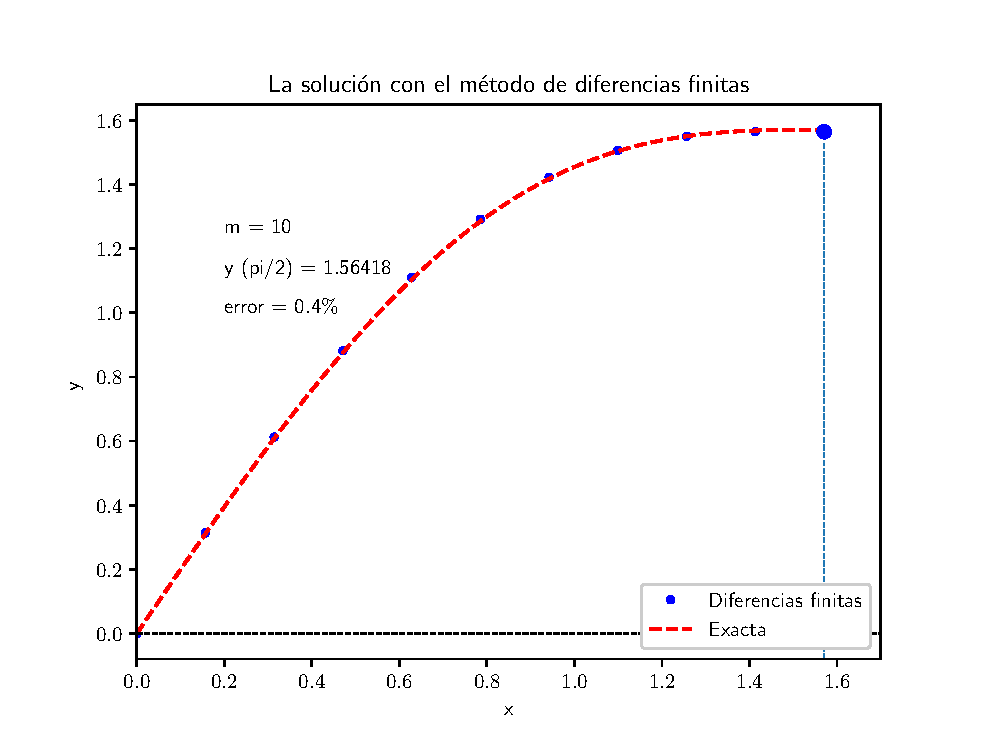
\includegraphics[scale=0.55]{Imagenes/plot_CDF_Dif_Fin_Ejercicio_01_01.eps}
\end{figure}
\end{frame}
\begin{frame}
\frametitle{Aumentando el valor de $m$}
Se logra una mayor precisión si se incrementa el valor de $m$.
\\
\bigskip
\pause
Repite el ejercicio con $m = 100$ y demuestra que el error relativo es del orden de ....
\end{frame}
\begin{frame}
\frametitle{La solución numérica}
\begin{figure}
    \centering
    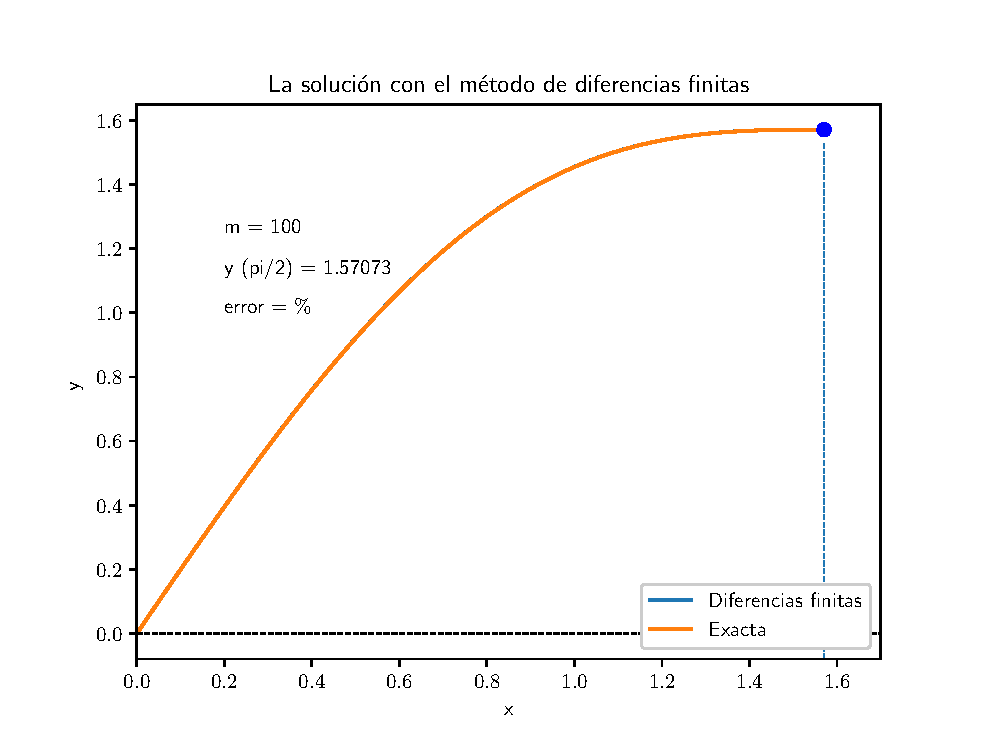
\includegraphics[scale=0.55]{Imagenes/plot_CDF_Dif_Fin_Ejercicio_01_02.eps}
\end{figure}
\end{frame}
\end{document}